\section{PMT testing, counter assembly and testing technical detail}

 %Look at section 11 "F Counter construction and testing process" for how to write this section.
% Copy the style of writing and maybe some of the procedures.

PMT Testing\\




For quality assurance of the photomultiplier tubes and counter assemblies used in the CLAS12 1b detector panel, a set of testing procedures was developed.  During the testing procedures some precautions were made in order to preserve the internal electronics of the PMTs.  In order to prevent overcurrent in the PMTs the high voltage was to never exceed \SI{1750}{V} and the PMT was never exposed to light while the high volatge was on.

The testing procedures began with unpacking the PMTs, connecting the high voltage cable to the power supply and the anode and dynode calbes to {\color{red}(**)} .  The PMT with attached cables was then loaded into the light tight testing box.\textit{\color{blue}Should there be a diagram?} In doing this the PMT was placed flush against the scintillator and affixed with optical grease in order to decrease light leakage.

A set of {\color{blue}baseline measurements} is conducted in order to 
\textbf{\color[rgb]{1,0.5,0}$\bullet$ Baseline measurements}\\
$\bullet$ Remove the source.\\
$\bullet$ Feed the anode signal into the Linear FiFo; one output going to the discriminator with a threshold of $10 mV$ and output directly to a visual scalar. The second output should go to the oscilloscope.\\
$\bullet$ For scalar measurements, remove the VETO for 100 seconds and record the count on the scalar\\
$\bullet$ For Oscilloscope measurements, set vertical scale to $20 mV$, adjust trigger to $10 mV$, and take a range of frequency values and average\\
{\color{blue}$\bullet$ Would like to see what these measurements are.}\\
$\bullet$ $1500 V$ ADC\\
$\bullet$ Record (ADC mean - offset mean).\\
$\bullet$ Perform 2 times.\\
$\bullet$ For ADC measurements use the voltage splitter at $1500 V$ even if not needed\\
$\bullet$ Baseline ADC\\
{\color{blue}$\bullet$ Is this supposed to be repeated?}\\
$\bullet$ adjust HV to baseline\\
$\bullet$ Record (ADC mean - offset mean).\\
$\bullet$ Perform 2 times.\\
$\bullet$ For ADC measurements use the voltage splitter even if not needed\\
$\bullet$ Baseline rate of events\\
{\color{blue}$\bullet$ Is this supposed to be repeated?}\\
$\bullet$ Feed the anode signal with source into Linear FiFo; one output going to the discriminator with a threshold of $10 mV$ and output directly to a visual scalar. The second output should go to the oscilloscope.\\
$\bullet$ For scalar measurements, remove the VETO for 100 seconds and record the count on the scalar\\
$\bullet$ For Oscilloscope measurements, set vertical scale to $20 mV$, adjust trigger to $10 mV$, and take a range of frequency values and average\\

\textbf{\color[rgb]{1,0.5,0} $\bullet$ Baseline dark current: How should these plots look?}\\
\begin{figure}[ht!]
\centerline{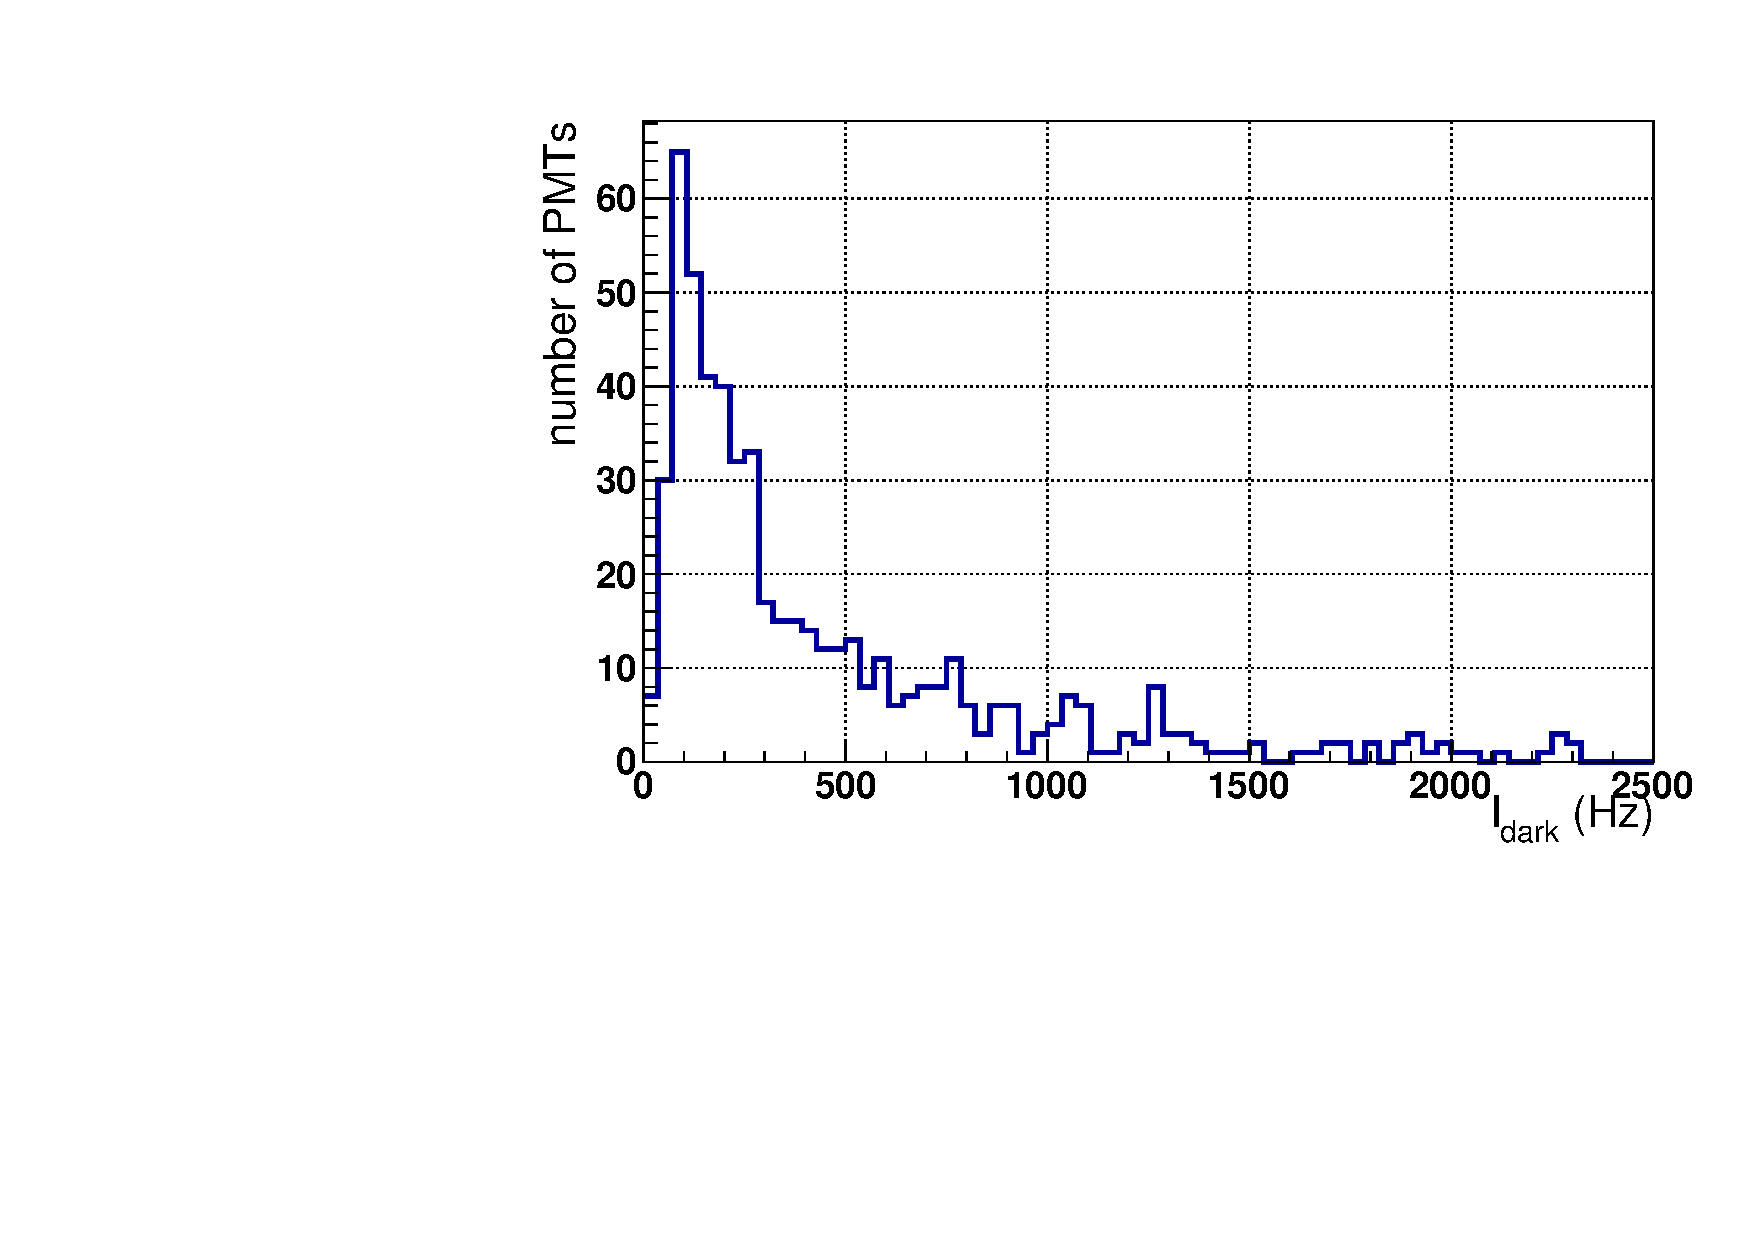
\includegraphics[width=8cm,height=6cm]{ye/fig_ye_pmt_test/dark_curr_measured.pdf}}
\caption{Measured dark current }
\label{f:dark_measure}
\end{figure}

\begin{figure}[ht!]
\centerline{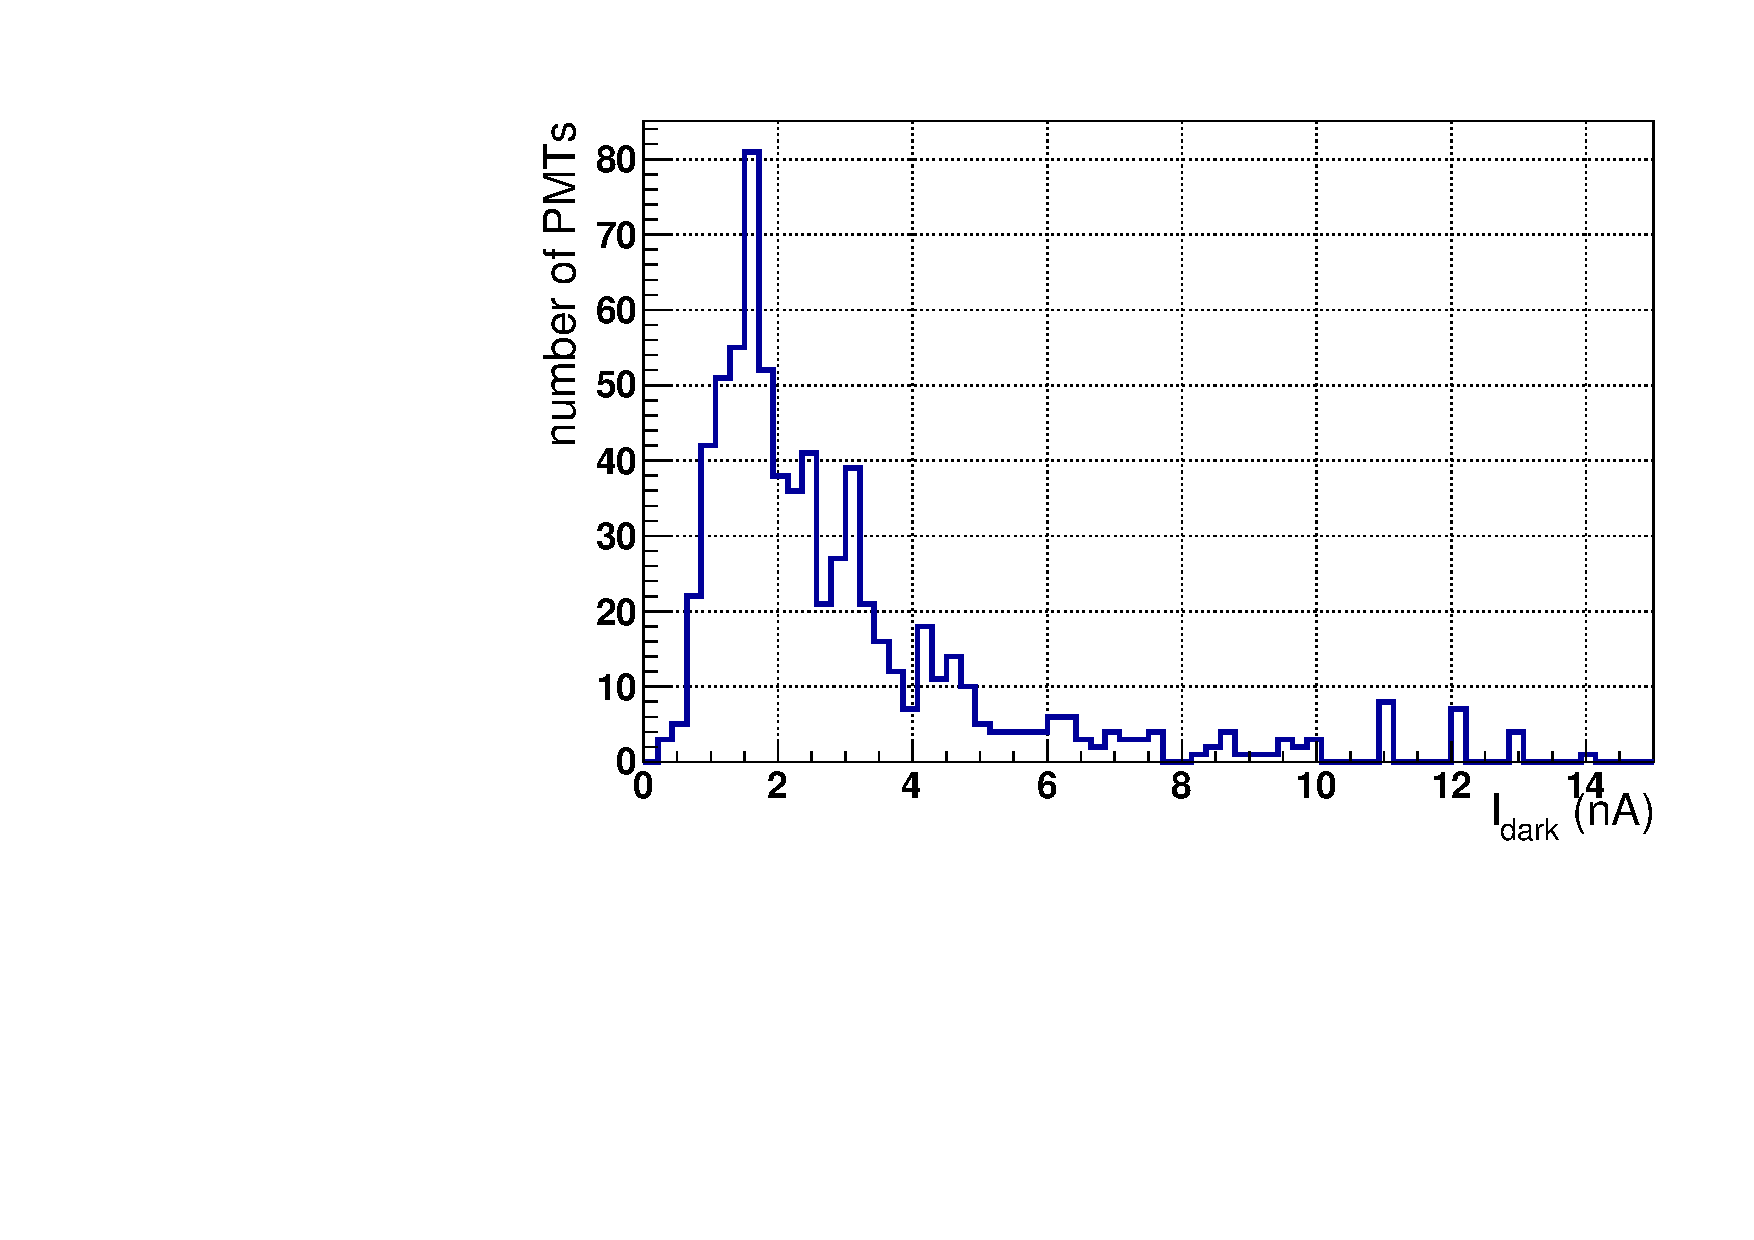
\includegraphics[width=8cm,height=6cm]{ye/fig_ye_pmt_test/dark_curr_factory.pdf}}
\caption{Factory dark current }
\label{f:dark_factory}
\end{figure}

\begin{figure}[ht!]
\centerline{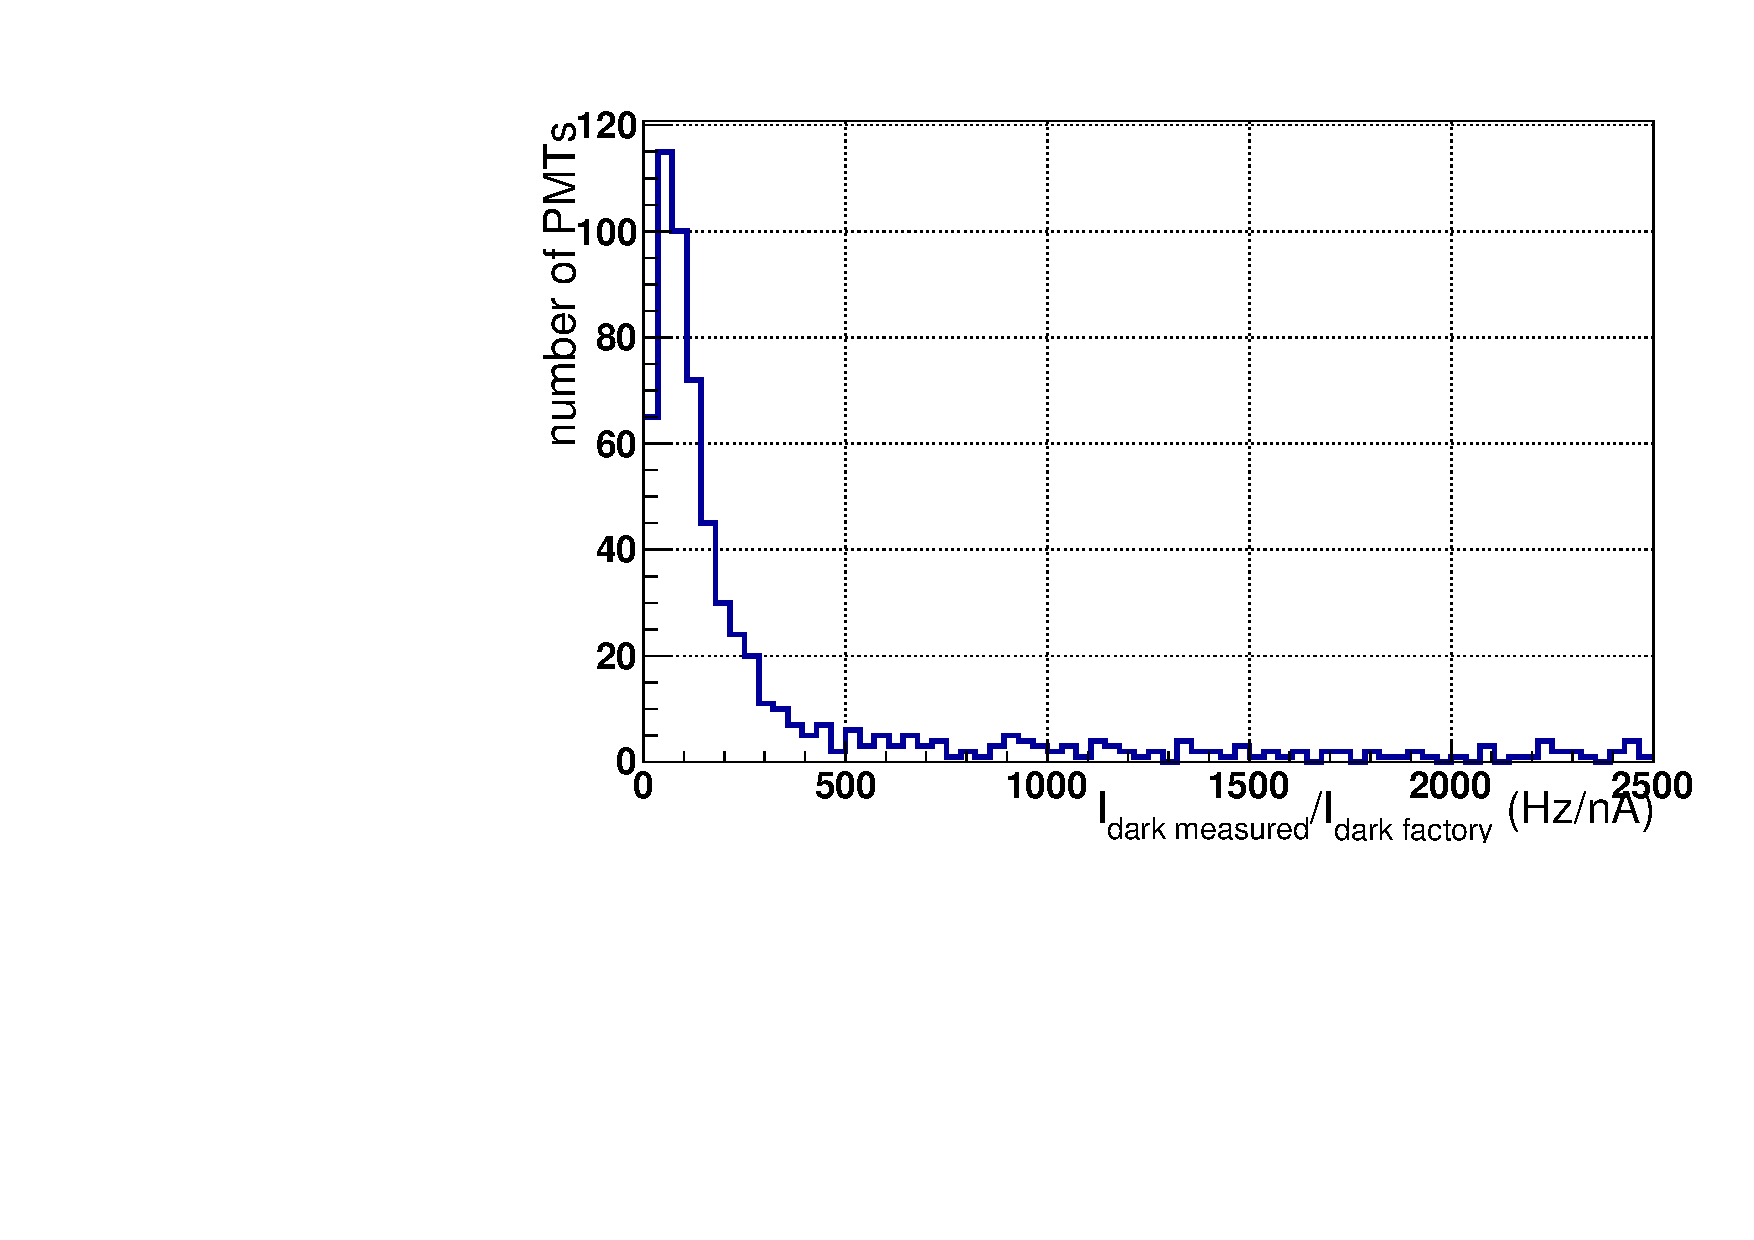
\includegraphics[width=8cm,height=6cm]{ye/fig_ye_pmt_test/dark_curr_ratio.pdf}}
\caption{Factory and measured dark current ratio }
\label{f:dark_ratio}
\end{figure}

{\color{blue}$\bullet$ Is this supposed to be repeated?}\\
{\color{blue}$\bullet$ What is different about each repeated measurement? What is each set of measurements for?}\\
{\color{blue}$\bullet$ Could this be stated once and then referred back to?}\\
$\bullet$ Feed the anode signal into the Linear FiFo; one output going to the discriminator with a threshold of $10 mV$ and output directly to a visual scalar. The second output should go to the oscilloscope.\\
$\bullet$ For scalar measurements, remove the VETO for 100 seconds and record the count on the scalar\\
$\bullet$ For Oscilloscope measurements, set vertical scale to $20 mV$, adjust trigger to $10 mV$, and take a range of frequency values and average\\

\textbf{\color[rgb]{1,0.5,0}$\bullet$ Baseline snapshot}\\
$\bullet$ 1500 snapshot\\
$\bullet$ 1700 snapshot\\
$\bullet$ 1500 rate of events\\
$\bullet$ Feed the anode signal with source into the Linear FiFo; one output going to the discriminator with a threshold of $10 mV$ and output directly to a visual scalar. The second output should go to the oscilloscope.\\
$\bullet$ For scalar measurements, remove the VETO for 100 seconds and record the count on the scalar\\
$\bullet$ For Oscilloscope measurements, set vertical scale to $20 mV$, adjust trigger to $10 mV$, and take a range of frequency values and average\\
$\bullet$ 1500 dark current\\
$\bullet$ Feed the anode signal into the Linear FiFo; one output going to the discriminator with a threshold of $10 mV$ and output directly to a visual scalar. The second output should go to the oscilloscope.\\
$\bullet$ For scalar measurements, remove the VETO for 100 seconds and record the count on the scalar\\
$\bullet$ For Oscilloscope measurements, set vertical scale to $20 mV$, adjust trigger to $10 mV$, and take a range of frequency values and average\\

\textbf{\color[rgb]{1,0.5,0}$\bullet$ Rise time}\\
$\bullet$ Plug into oscilloscope and read off the numbers\\
$\bullet$ Note: All measurements using the splitter or attenuators will result in values that are one half (for the splitter) or a fraction of (variable based on the attenuator) their actual value\\
$\bullet$ Add test results and notes to corresponding database entry. All measurements should have corresponding Oscilloscope snapshots and histograms where applicable.\\
$\bullet$ Remove any grease from black box at end of day.\\
\begin{figure}[ht!]
\centerline{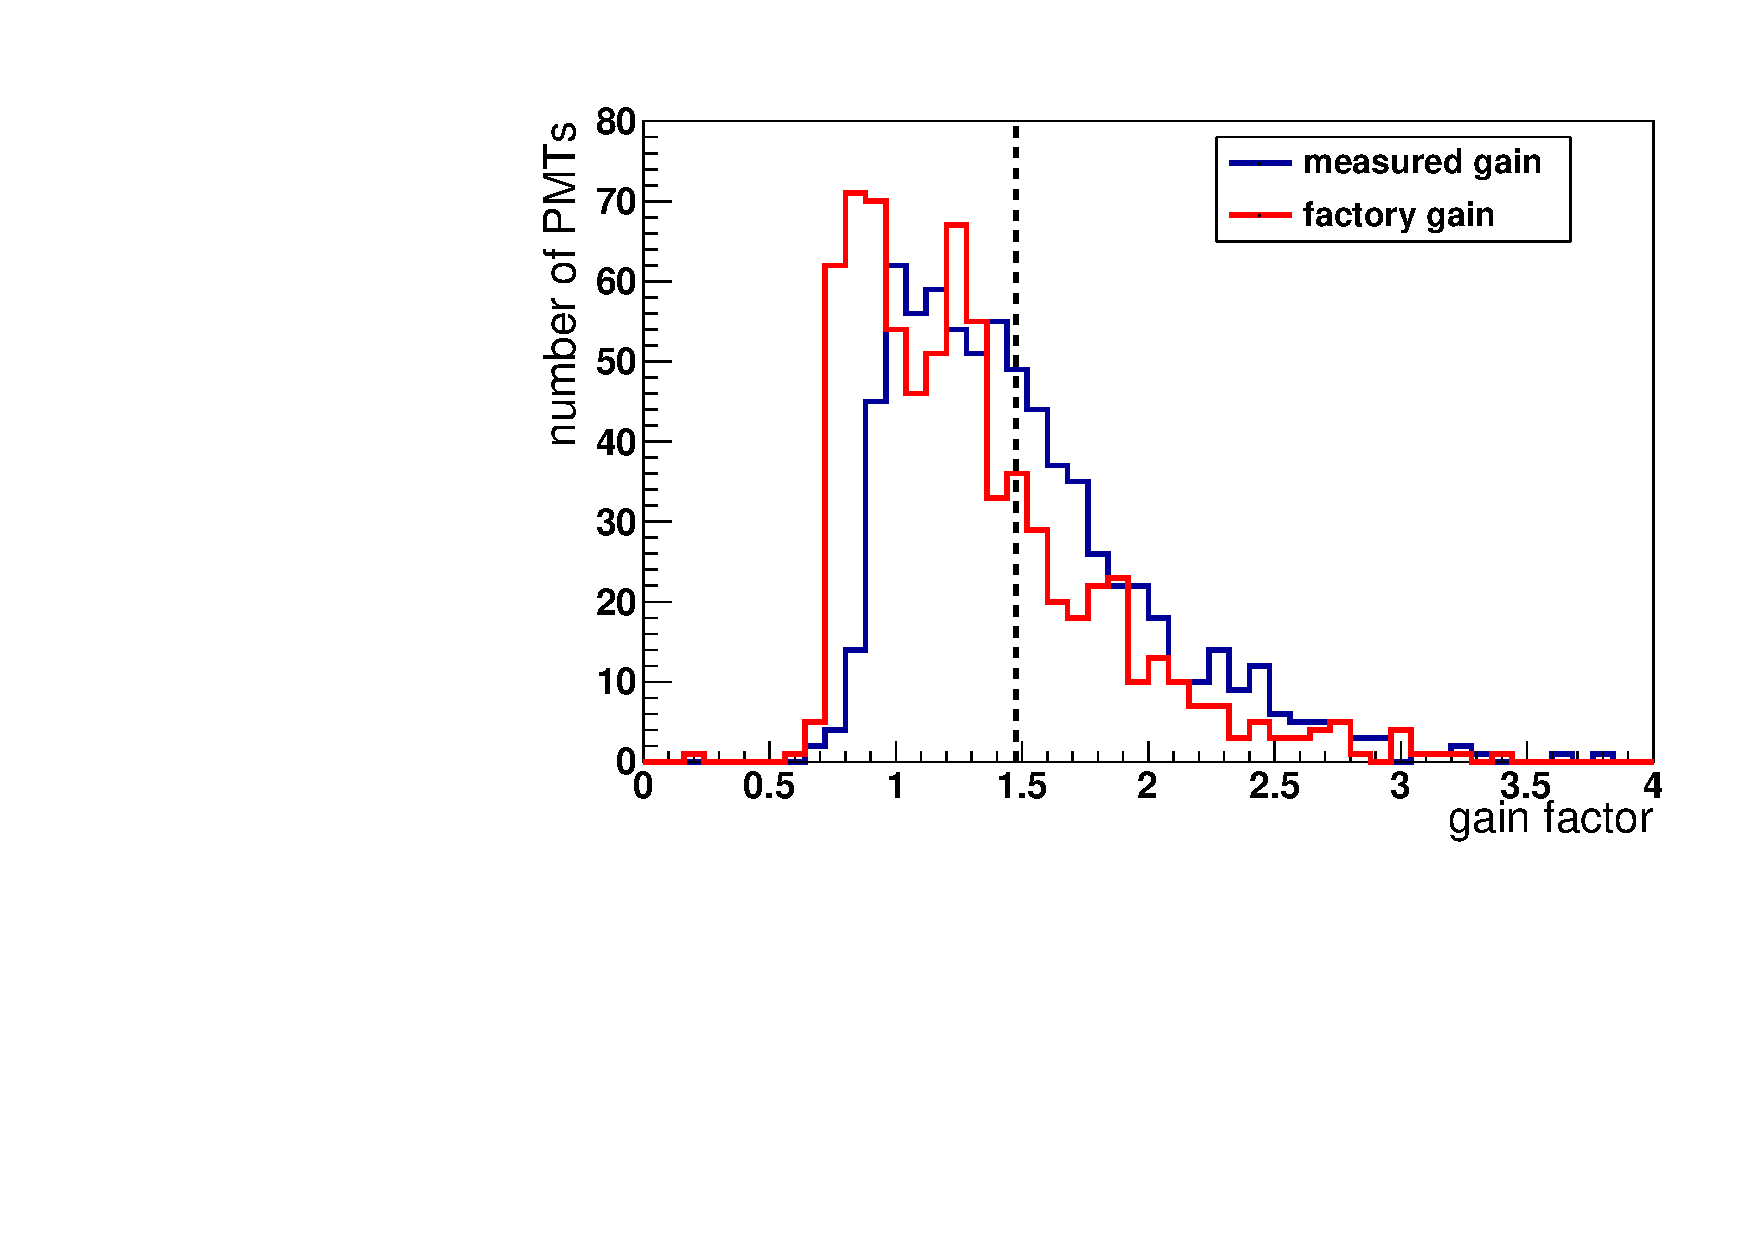
\includegraphics[width=8cm,height=6cm]{ye/fig_ye_pmt_test/gain.pdf}}
\caption{gain}
\label{f:gain}
\end{figure}


\begin{figure}[ht!]
\centerline{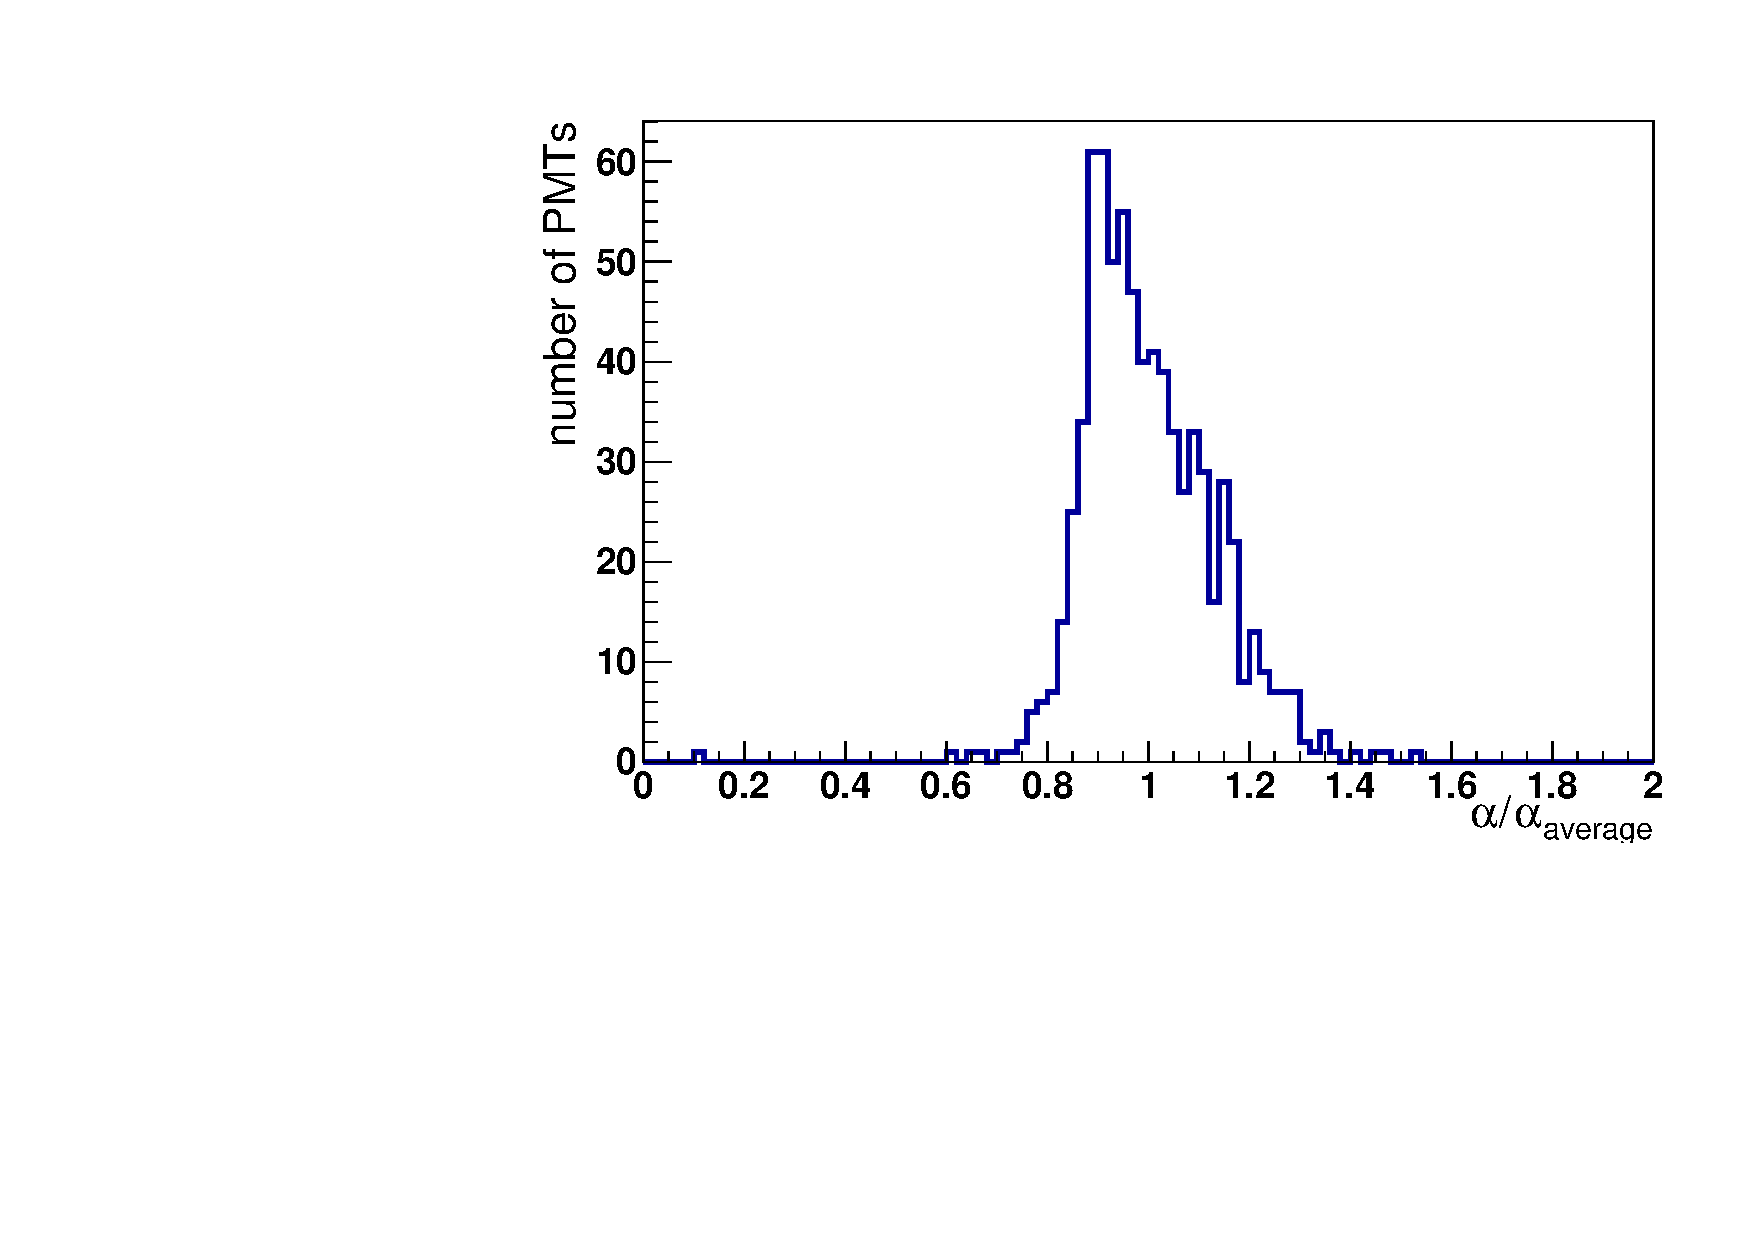
\includegraphics[width=8cm,height=6cm]{ye/fig_ye_pmt_test/alpha.pdf}}
\caption{alpha}
\label{f:alpha}
\end{figure}

\textbf{\color[rgb]{1,0.5,0}Counter Assembly}\\
$\bullet$ Crew size: 2-3, depending on length.\\
$\bullet$ Prepare and clean workbench area, and retrieve six identical-length scintillators from storage area.\\
$\bullet$ Use latex gloves before further handling the scintillators.\\
{\color{blue} $\bullet$ Grease and oils from hand have different reflective properties creating anomalies in further measurements? Can oils ruin scintillators? Could this be included in warnings section at top?}\\
$\bullet$ Remove protective film only at the end faces of the scintillators.\\
$\bullet$ Each end of the scintillator is fitted with black tape (hereon referred to as ``anticookie''), which masks the corners while leaving a circular window that extends one millimeter into the area that will be covered by the PMT. Apply anticookie end window.\\
$\bullet$ Mask the scintillator around top edges of protective tape with electrical tape slightly above the top edge. Fold the tape down to prevent glue dripping.\\
$\bullet$ Place the scintillators Diamond cut side facing you horizontally into the
windmill frame while maintaining a balanced load.\\
$\bullet$ Pressurize the air pistons to $40$ psi to secure the scintillators in place.\\
$\bullet$ Use the hydraulic lift to raise the windmill frame, clearing it for rotation, and
rotate so that the scintillators are vertically aligned.\\
$\bullet$ Secure height and rotation angle, and keep the compressor powered.\\
$\bullet$ Mount centering tool with open side facing you. Leave a $1.5\;cm$gap between
the top of the scintillator and the centering tool for easy centering.\\
$\bullet$ Extract $7.4 \;ml$ of each of scintillator glue and $2.4\; ml$ of catalyst using disposable syringes and squirt the content into a disposable mixing container.\\
$\bullet$ Mix and pour glue into a capped syringe with its stopper removed and mount it into one of the base holes in the vacuum chamber and seal.\\
$\bullet$ Close all valves and open valve to chamber from pump. Evacuate chamber to
 $30$ psi. Close valve, turn pump off, and wait for 2 minutes. Open release valve on pump farthest from chamber to protect pump from condensation. Open release valve on chamber to restore pressure, and wait 2 minutes. Close all valves.\\
$\bullet$ Wrap paper towel around bottom base of centering to catch excess glue.\\
$\bullet$ Prepare PMT for gluing.\\
$\bullet$ Place stopper in syringe and squeeze out any remaining air from tip.\\
$\bullet$ Apply approximately $1 ml$ of glue to the top end of a scintillator, straight down in the center of the anticookie.\\
$\bullet$ Check for bubbles in glue. If bubbles are found reapply glue.\\
$\bullet$ Lower the PMT in a rotating motion through the centering tools slowly onto the scintillators ensuring that copper on PMT points to front left corner.\\
$\bullet$ Continue process until all PMT's are mounted checking the syringe for any glue bubbles near the tip. If glue bubbles are present in the syringe you must remix new glue to ensure there are no bubbles.\\
$\bullet$ Using an Allen wrench set width of centering tools to center PMT if needed.\\
$\bullet$ Look in open area of centering tool to make sure the PMT is centered, then center between diamond-tooled side with gloved fingers. Re-verify centering of molded side with eyes.\\
$\bullet$ Distribute 3 wires evenly about PMT.\\
$\bullet$ After at least 12 hrs, rotate the windmill frame with the scintillators by $180^{\circ}$, and repeat the gluing process.\\
$\bullet$ After at least 12 hrs, rotate the windmill frame into the horizontal, turn off the air compressor, and release the pressure.\\
$\bullet$ Prepare and clean workbench area, and move one counter onto the workbench.\\
$\bullet$ Create a single counter label that includes the manufacturer-provided identification numbers for the scintillator and the PMT's, as well as a position dependent number i from 1, most inner and shortest, to 64, most outer and longest scintillator.\\
$\bullet$ Check that PMT orientations align with each other.\\
$\bullet$ If the PMT's do not align with each other they must be re-glued.\\
$\bullet$ If the PMT's align with each other but are offset from center you may continue.\\
$\bullet$ File the corners of the diamond cut ledge to further protect wrapping.\\\
$\bullet$ File the corners smooth with a fine file.\\
$\bullet$ Blow scintillator with compressed air to remove dust.\\
$\bullet$ Remove black electric tape from ends of scintillator.\\
$\bullet$ Remove protective film, keep track of the new counter label, and remember that
you will not be able to attach the new label until the entire wrapping procedure
is concluded.\\
$\bullet$ Perform detailed scintillator visual inspection, and record all inclusions,
bubbles, scratches, cloudy areas, refraction index changes, or any other
anomalies with their respective sizes and coordinates.\\
$\bullet$ Identify diamond-tool-finished (defining the height) and molded (defining the
width) sides. The molded side should be face up and defines the front of the
scintillator.\\
$\bullet$ For previously non-centered but aligned PMT pairs it will be important to orientate the bar such that the side with the greatest gap between the PMT and the edge of the bar be face up denoting the front of the scintillator.\\
$\bullet$ File corner edges of scintillators to protect light tight wrapping. Using a flat coarse file file the corner down $4 mm$; Only file away from the anticookie during this step.\\
$\bullet$ Log progress in check sheet.\\
$\bullet$ Cut the Mylar film to length, and wrap the counter in a single layer. Apply the transparent tape only on one molded side, which so defines the front side.\\

$\bullet$ Trim the Mylar film to the length of the scintillator.\\
$\bullet$ Cut the Tedlar film in half with the spool-mounted cutting tool.\\
$\bullet$ Cut the Tedlar film to length (scintillator length plus $20 cm$ on each end), and wrap the counter tightly and wrinkle-free in three layers. Retain the film tension with electrical tape, secured only on the front side. Finish it off with a layer of the $5 cm$ wide, thin, black tape running the full length of the Tedlar sheet.\\
$\bullet$ Apply the counter label to the center of the front side and cover with evenly cut clear tape.\\
$\bullet$ Record width and height every $20 cm$ and the overall length and straightness. Verify whether they are within specifications. Add inspection notes and measurements to corresponding scintillator database entry.\\
$\bullet$ Wrap 2 layers of electrical tape around PMT $3 cm$ from edge of scintillator and at end near wires.\\
$\bullet$ Firmly pigtail the Tedlar film as close as reasonably possible to the PMT HV divider in the center with the electrical tape, trim the Tedlar to $3 cm$ from the PMT HV divider, and finish the pigtail by wrapping the electrical tape around the bundled Tedlar and cables extending to $5 cm$ beyond the PMT HV divider.
$\bullet$ Check that the ends closest to the PMT of the Tedlar pigtail are less than $15.5mm$ in diameter.\\
$\bullet$ Zip tie wires tightly using pliers at base of PMT and trim excess.\\
$\bullet$ Blow work area clear before starting new bar.\\
$\bullet$ Before loading the first bar into the six-bar testing rack, ensure that the previous counter control measurement has been signed off. If the rack is still loaded, stop the measurement, turn off the individual HV channels, unplug the HV, anode, and dynode cables, and unload the six-bar rack, storing each counter on the designated shelf in the storage area.\\
$\bullet$ Load the counter into the six-bar testing rack with the bottom side facing the wall.\\
$\bullet$ Add the new counter in the database by associating the entries of the two PMT's
with that of the scintillator.\\
$\bullet$ Repeat the inspection and wrapping procedure for the remaining scintillators.

\textbf{\color[rgb]{1,0.5,0}Counter Control Measurements}\\
$\bullet$ Ensure that the six counters are properly aligned and secured in the six-bar rack.\\
$\bullet$ Connect HV, anode, and dynode cables, each set from top-left, labeled 1 to bottom-right, labeled 12.\\
$\bullet$ Apply baseline voltages according to PMT testing task database entries.\\
$\bullet$ Verify that the anode and dynode signals on the oscilloscope match the nominal documented pulse-shape distribution.\\
$\bullet$ Verify that the dark current is independent of light on/off status.\\
$\bullet$ Start LabVIEW VI ``Calibration Stack Reader.vi'' to begin Calibration run.\\
$\bullet$ Start LabVIEW VI ``Histogram Grapher.vi''. Check that channels match PMT's on the first tab labeled Data map and press confirmation button.\\
$\bullet$ Move to the ADC tab and plot histograms by holding down the ``Plot ADC DATA'' button. Adjust voltage till histograms leading edge lines up with read line on all graphs. Restart both programs between each run.\\
$\bullet$ Move to TDC tab and check for consistency between each channel. If not consult task expert.\\
$\bullet$ Further help is available by pushing the Instructions button in the lower left corner of program or ask the task expert if any discrepancies remain.\\
$\bullet$ Close previous VIs and Start the LabVIEW VI ``24 hour ComboStackReader.splitter.noproc.vi'' to start a 24 hour run. First create a file name specific to your current task by pressing the ``Enter File Name'' button then hit start.\\
$\bullet$ Enter your name on screen.\\
$\bullet$ Enter your name and start time in the log book at the computer station.\\
$\bullet$ The program will run for 24 hours then create a new file every subsequent day automatically until stopped. A green light will turn on when the first 24 hours has passed. The automated analysis system will automatically process the collected data and store the results and histograms into the database when the run is complete.\\

\textbf{\color[rgb]{1,0.5,0}Counter Control Analysis and Sign-off}\\
$\bullet$ Verify that the automated analysis process is complete and that the corresponding files and database entries are present.\\
$\bullet$ Verify control histograms and spot-check database entries according to interactive checklist application, as described in more detail in Section f, Quality Assurance Plan, of this document.\\
$\bullet$ At the end of the interactive checklist, the application will request sign off and will store all responses with the user's id.\\
$\bullet$ If sign off is not warranted, the task expert must be consulted for resolution. Backing Structure and Two-Counter Assembly\\
$\bullet$ Prepare and clean workbench area, and retrieve an odd-i backing structure\\
$\bullet$ Consult database and diagram to find corresponding counters, $i$ and $i+1$.\\
$\bullet$ Retrieve a pair of both the left and right stoppers, 16 screws, and, if required by the assembly plan, 4 mu-metal shields.\\
$\bullet$ Add a new two-counter assembly to the database by associating these two counters and this backing structure.\\
$\bullet$ Mount left stoppers for sectors 3, 4, and 5 in their most outward positions and for sectors 1, 2, and 6 with screws slit-centered.\\
$\bullet$ Mount right stoppers for sectors 1, 2, and 6 in their most outward positions and for sectors 3, 4, and 5 with screws slit-centered.\\

\textbf{\color[rgb]{1,0.5,0} Backing Structure} \\
$\bullet$ Prepare the backing structure for taping by first marking the placement for taping onto the structure itself. Refer to the overall diagram for the taping pattern for the current backing structure. The tape-loop pairs are at intervals of $40 cm$ for long counters and $20 cm$ for short counters ($30 cm$ gap between tape loop pairs). Mark additional single loops at each end following the pattern on Fig.~\ref{sector3135}.\\
\begin{figure}[h!]
\centerline{
\includegraphics[width=13cm,height=3cm]{ye/fig_ye_pmt_test/sector-31-35.pdf}}
\caption{Final taping structure of all sectors }
\label{sector3135}
\end{figure}
$\bullet$ Apply the single-sided rubber tape to the front of the backing structure in the $30 cm$ gap between the tape-loop pair markings. The rubber tape should be measured out to $29 cm$ and placed directly between tape-loop pairs with a half cm tolerance to the loop pairs.\\
$\bullet$ Suspend the backing structure between 2 stools/sawhorses and clamp it to them. This will allow you to freely tape the structure.\\
$\bullet$ Prepare tape-loop pairs, starting from the center of the backing structure. Tape loops of adjacent backing structures must be offset to avoid overlap, so backing structures 1, 5, 9, ... must have tape-loop pairs starting at the center, and 3, 7, 11, ... must have two central tape-loop pairs equidistant from the center ($15 cm$). Place the tape-loop pairs in the areas previously marked for them . Each long (short) pair consists of two $5 cm x 65 cm (2.5 cm x 65 cm)$ bi-directional, double-sided fiberglass tape loops, running side-by-side extending from the back corner along the back, the side, and then across the top surfaces in opposite directions, the remaining length should overhang in preparation for the two counter pairs, as diagrammed on Fig.12, and displayed in the work area.\\
$\bullet$ An additional single tape loop must be added to the far ends of each backing structure. The loop orientation (left-handed or right-handed) will depend on the large full diagram.\\
$\bullet$ Place the longer counter onto the backing structure and orient it into its proper position. Lay the smaller counter next to it and mark its proper position onto the larger counter. This will act as a guide when taping them together.\\
$\bullet$ Caution: Tape is extremely adhesive and must be handled with care, and placed accurately. Apply the double-sided, high-tack polyester film tape along the length of the top diamond-tool-finished scintillator side of the shorter, lower, odd-numbered counter, remove the tape's protective film, and center and attach the bottom diamond-tool-finished scintillator side of the longer, upper, even numbered counter using the marks as a guide.\\
$\bullet$ Remove the protective film of the tape loops.\\
$\bullet$ Place the two-counter unit onto the backing structure, ensuring that it is positioned so that the edge of each counter's scintillator is $1 mm$ from the stoppers that have slit-centered screws.\\
$\bullet$ Continue by tightly wrapping each tape loop's remaining length around the two counter unit and back under the backing structure, completely overlapping with the first segment of the tape loop. Work as a team simultaneously on opposing tape-loop pair sides to avoid Tedlar wrinkles, especially on the top and bottom diamond-tool-finished sides, which will be stacked.\\
$\bullet$ Finish each tape-loop pair by applying a $12.7 x 53 cm^{2}$ single-sided, red Mylar tape loop, with both ends terminating on the back of the backing structure, to over the double-sided fiberglass tape.\\
$\bullet$ Ensure that the slit-centered stoppers are placed and secured at $1 mm$ from the scintillator end faces, and re-position the most outward-mounted stoppers at $5 mm$ from the opposite scintillator end faces.\\
$\bullet$ Store the backing structure counter assembly in the designated storage area.